% !TeX root = ../main.tex
\chapter{仿真实验}
仿真实验分为三步,首先在Matlab中基于s-function和simulink仿真,验证控制算法的性能;然后在ros框架下,基于PX4固件,修改其运动控制部分的代码,在gazebo中仿真;接着,将修改后的PX4固件烧写到pixhawk飞控板中,进行硬件在环仿真,而这个版本的固件也可以直接用于后续的实机实验。
\section{Matlab仿真}
我们在Simulink环境下构建了一个综合仿真模型,该模型不仅包含了刚体动力学和电机动态,还通过s-function实现了姿态环和位置环分离的双环控制器设计。这种设计使得后续的数据分析和研究工作能够更为便捷、高效。

为了能直观地体现性能,我们设计了一个“8”字型轨迹:
$$x_d = \begin{matrix}[4\sin(\frac{t}{3}), & 4\cos(\frac{t}{3})\sin(\frac{t}{3}), &-0.1t]\end{matrix}
\quad
\psi_d=0.01t$$

为了全面体现控制算法的跟踪性能,我们并没有对轨迹做特殊的平滑处理,轨迹的导数存在间断点使得高阶导数无穷大,这可以考验无人机在现实中的抗扰性能。为了模拟起飞和悬停,第一秒内轨迹保持在原点不动,否则仿真就会等同在空中释放电机无转速的无人机。

\begin{figure}[!h]
    \centering
    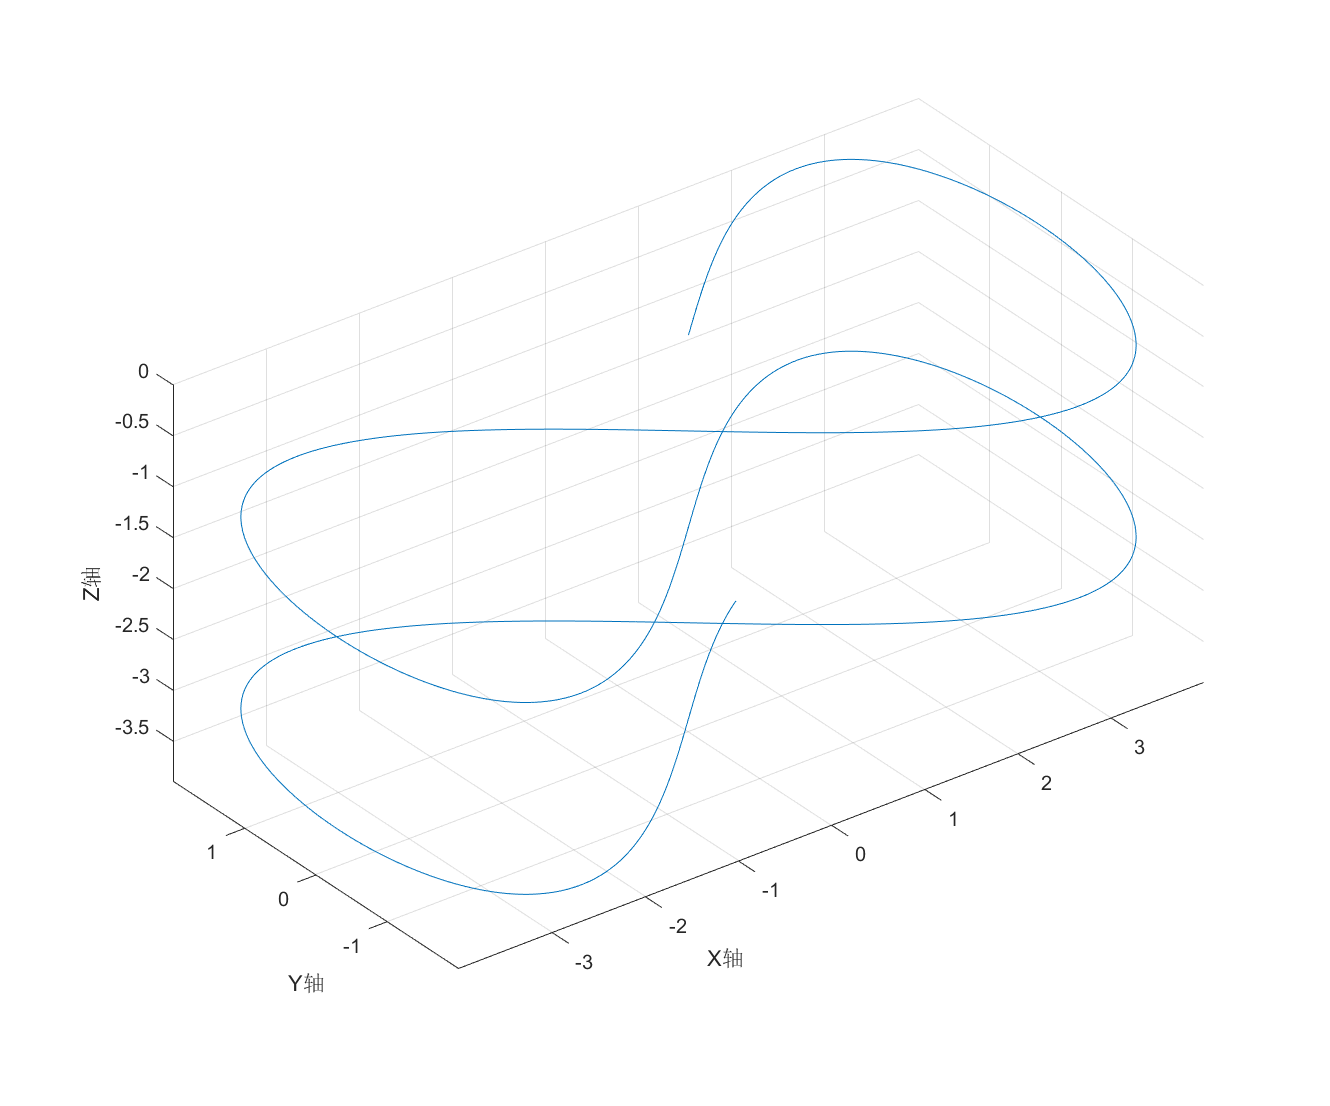
\includegraphics[width=0.65\textwidth]{88.png}
    \caption{高度匀速上升的“8”字型轨迹(北-东-地坐标系下,地面以上Z轴为负数)}
    \label{fig:8}
  \end{figure}

  无人机的刚体动力学部分由simulink中自带的“6DOF block”解决,避免了$SO(3)$群差分近似后单位化的困难。该模块会对外部输入的力和力矩做出反应,返回所需的速度、位置、姿态、角速度等信息。

  电机部分,转速的动态由一阶惯性环节表示,根据所选电机型号时间常数$\tau=0.01s$。
  姿态控制器和位置控制器分开由两个s-function实现,重力由单独的模块输入到“6DOF block”。
  \begin{figure}[!h]
    \centering
    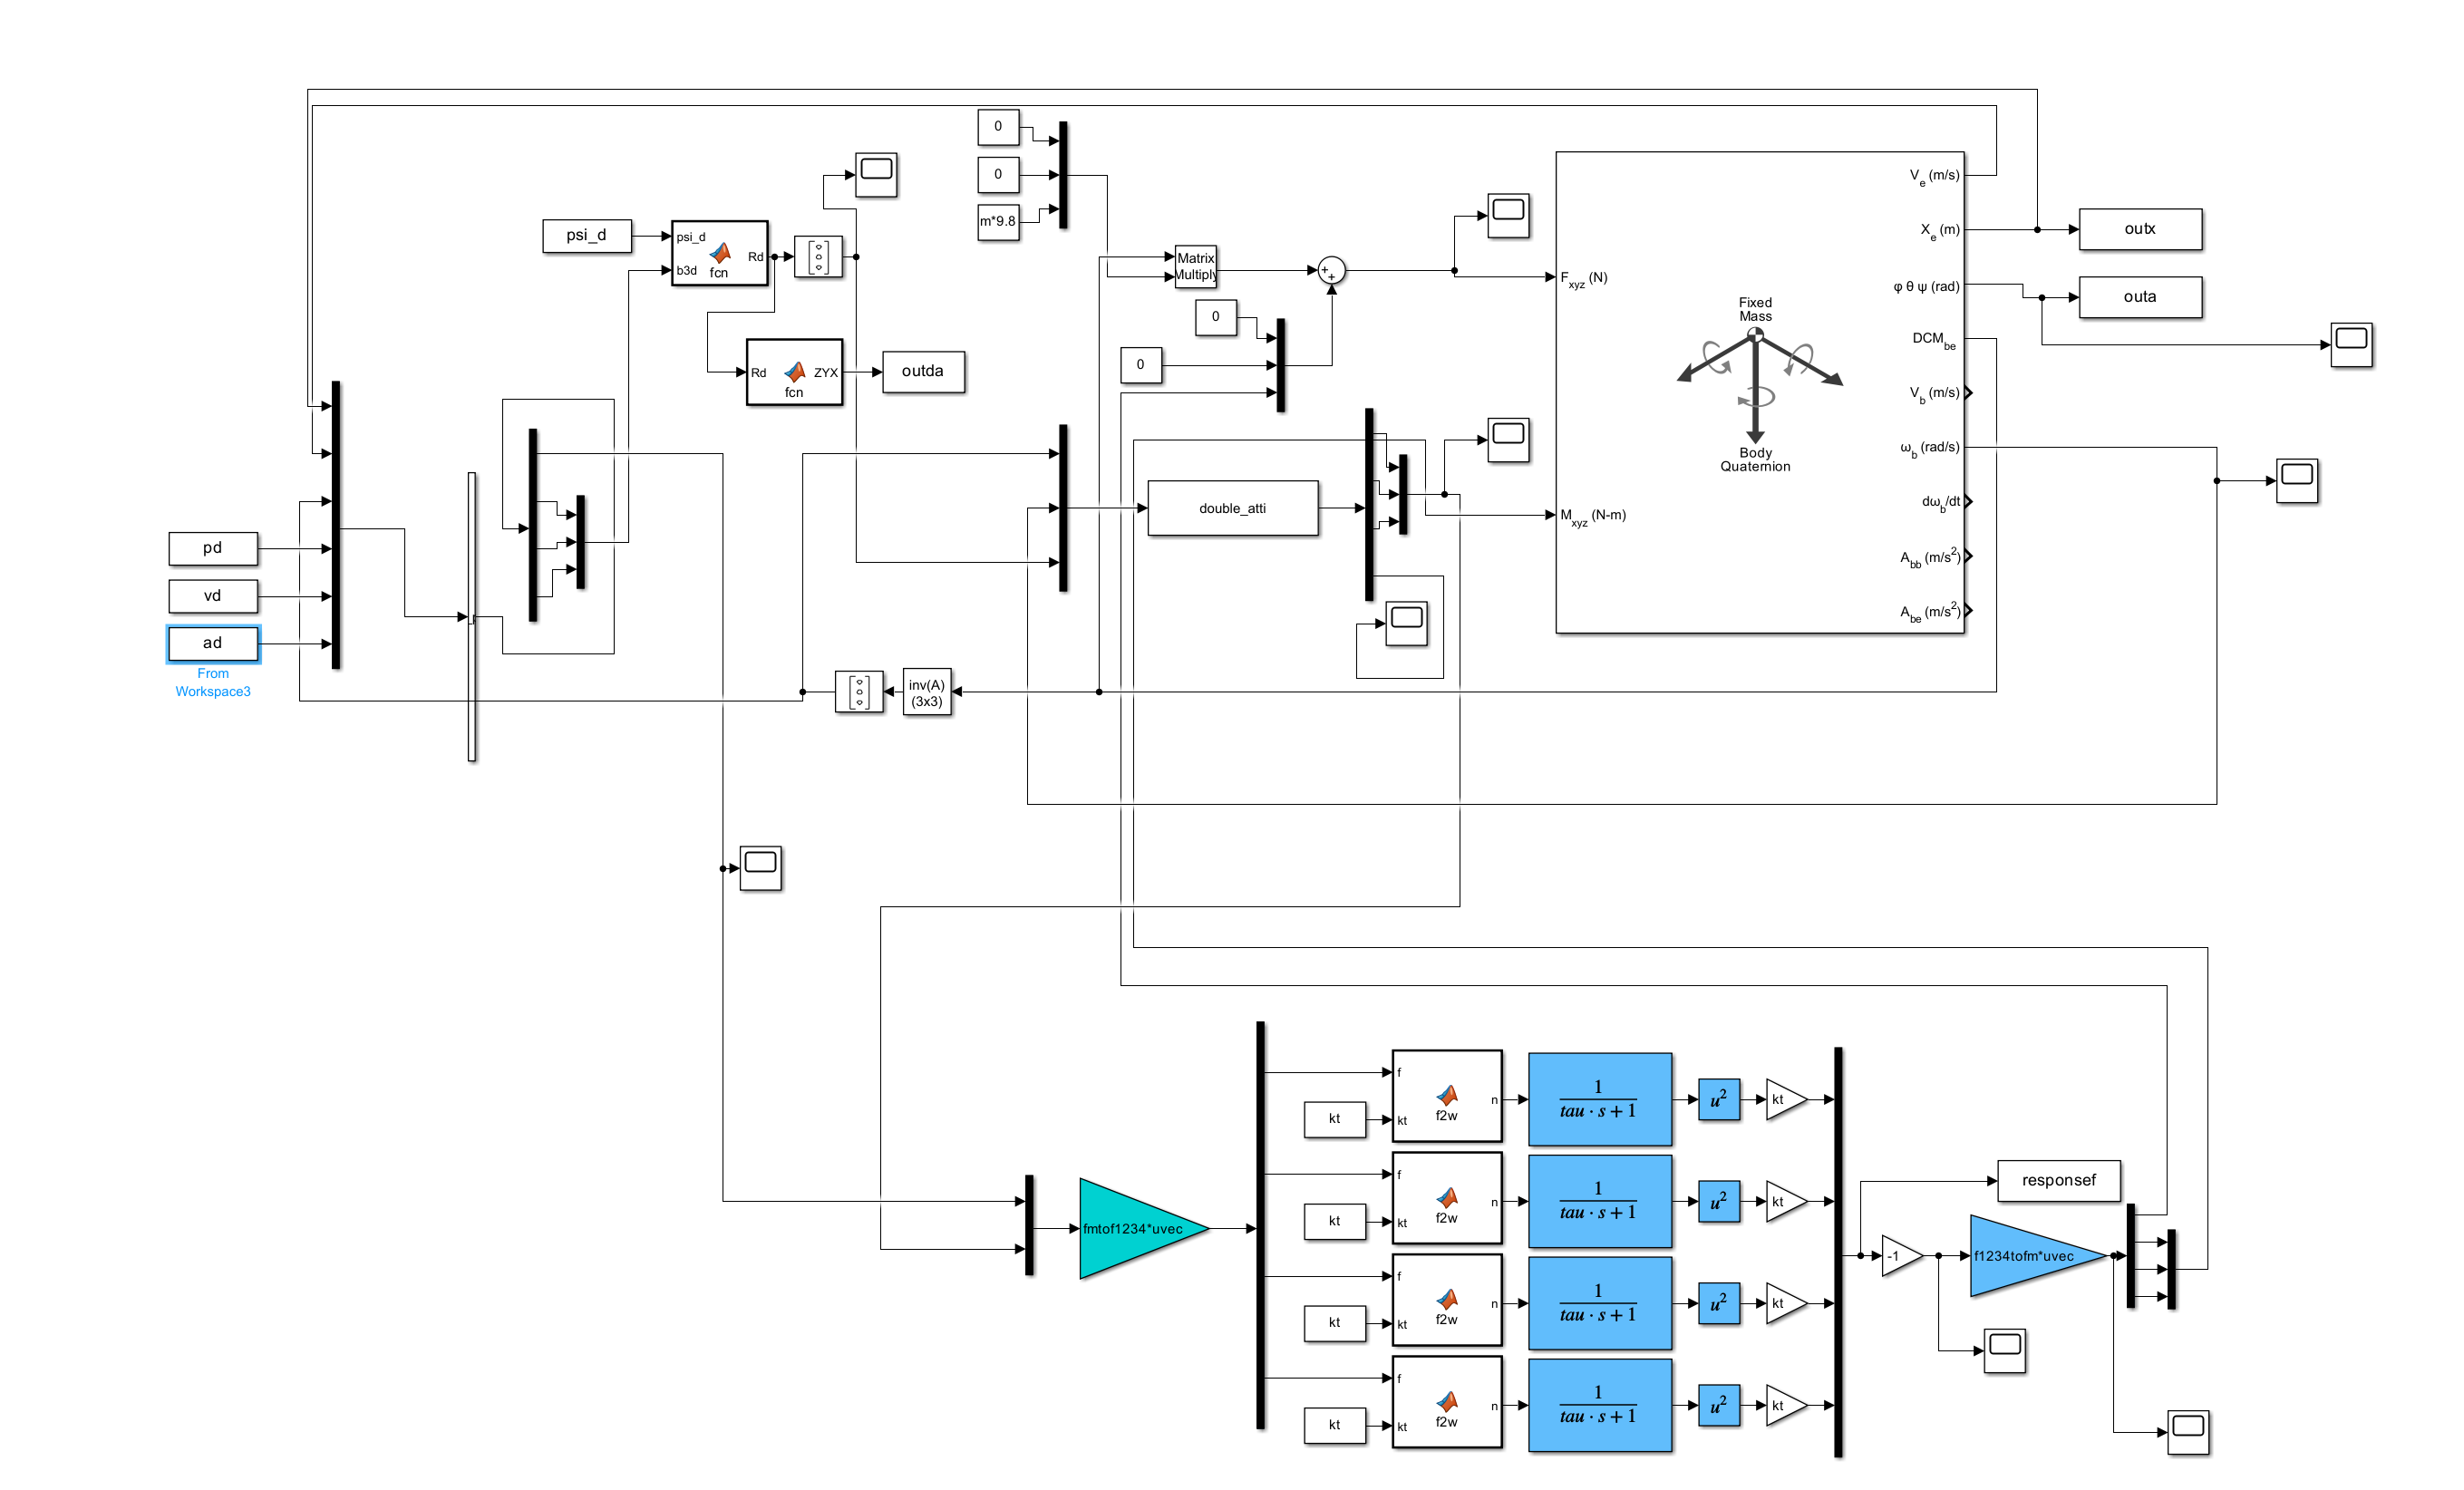
\includegraphics[width=0.9\textwidth]{sim.png}
    \caption{simulink仿真连线图}
    \label{fig:sim}
  \end{figure}

  四旋翼无人机的参数由测量和理论计算共同得到:
  $$m=0.8kg \quad d=0.125m \quad J=\begin{bmatrix}
    0.0024   &      0  &       0\\
    0 &   0.0025      &   0\\
    0  &       0   & 0.0041
  \end{bmatrix}kg m^2$$

  电机参数由厂家数据得到:
  $$k_t=2.03\times 10^{-8} \quad 
  \tau=0.01s \quad
  c_{\tau f}=8\times 10^{-3}$$

  选择替补姿态控制律:
  $$k_R=0.881 \quad k_\omega=0.254$$

  由于位置环和姿态环补偿后得到的线性系统A矩阵完全一致,因此选择相同的LQR权重矩阵:
  $$Q=\begin{bmatrix}
    3&0&0&0&0&0\\
    0&3&0&0&0&0\\
    0&0&3&0&0&0\\
    0&0&0&1&0&0\\
    0&0&0&0&1&0\\
    0&0&0&0&0&1\\
  \end{bmatrix} \quad R=\begin{bmatrix}
    0.1 &0 &0\\
    0 &0.1 &0\\
    0 &0 &0.1\\
  \end{bmatrix}$$

  初始位姿:
  $$x(0)=[0,0,0],\quad v(0)=[0,0,0]$$
  $$R(0)=I , \quad \omega(0)=[0,0,0]$$

  \begin{figure}[!h]
    \centering
    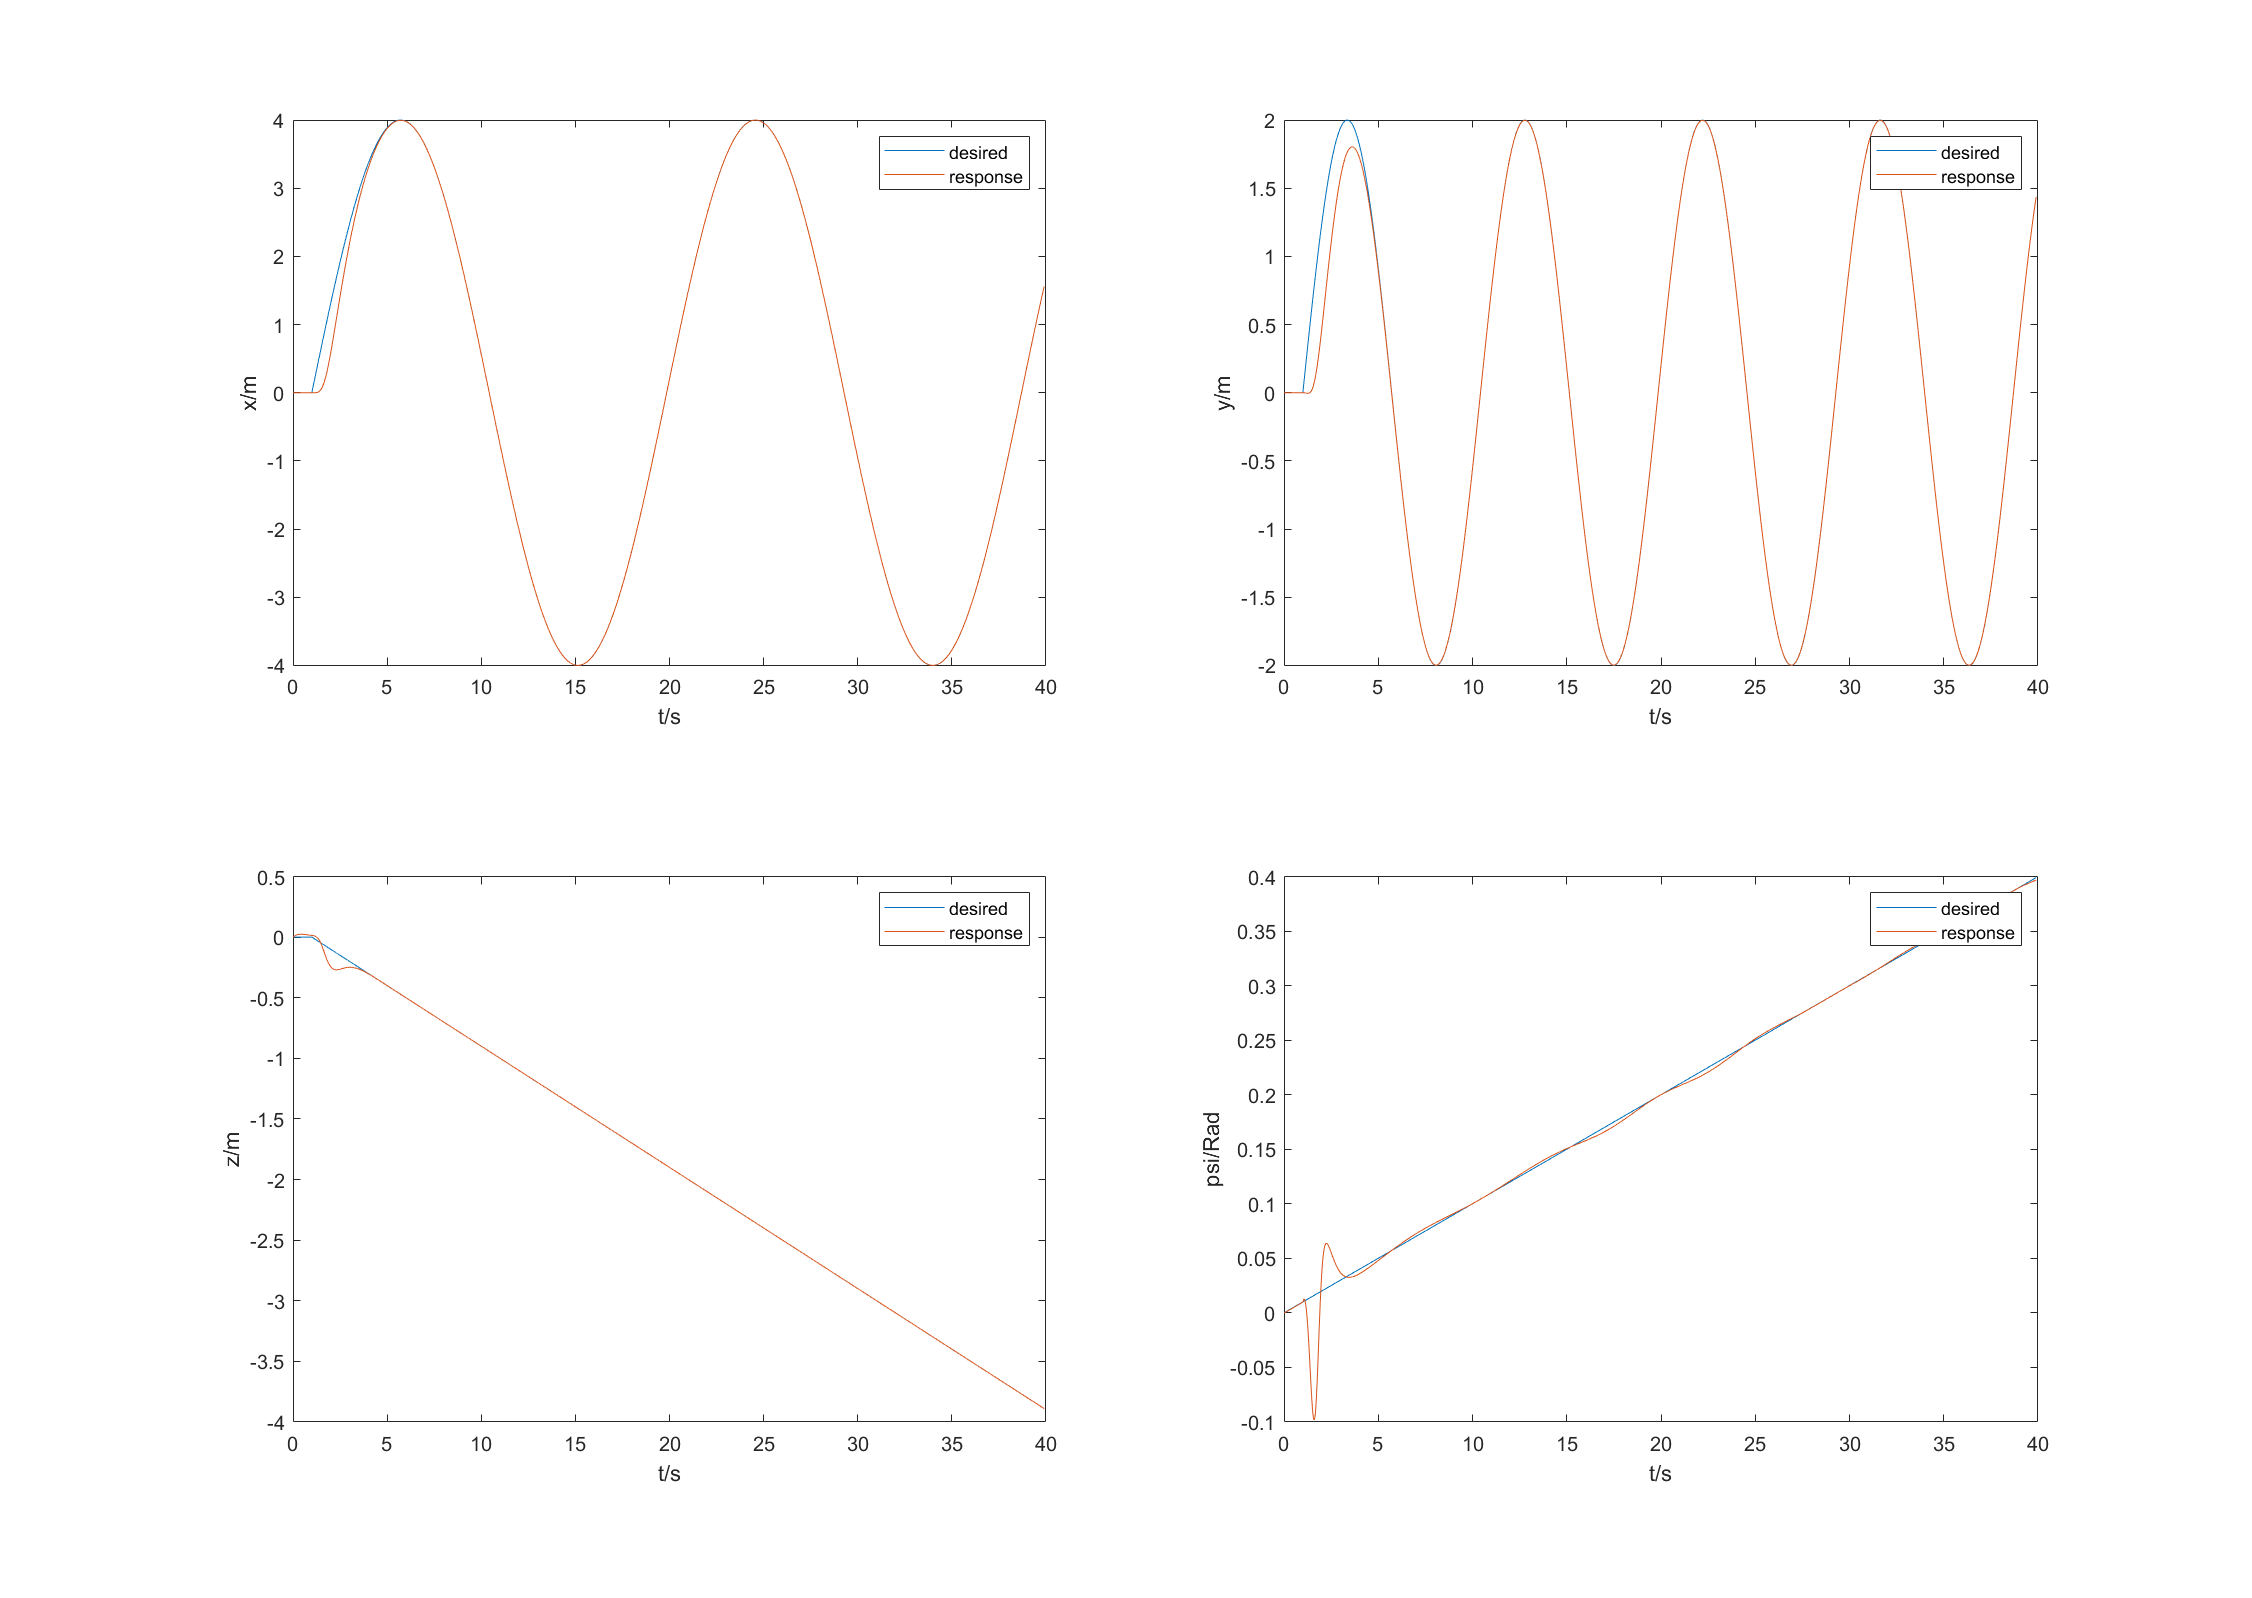
\includegraphics[width=0.9\textwidth]{result1.png}
    \caption{仿真实验结果:a) X轴跟踪曲线 b) Y轴跟踪曲线 c) Z轴跟踪曲线 d) 偏航角跟踪曲线}
    \label{fig:result1}
  \end{figure}

  \begin{figure}[!h]
    \centering
    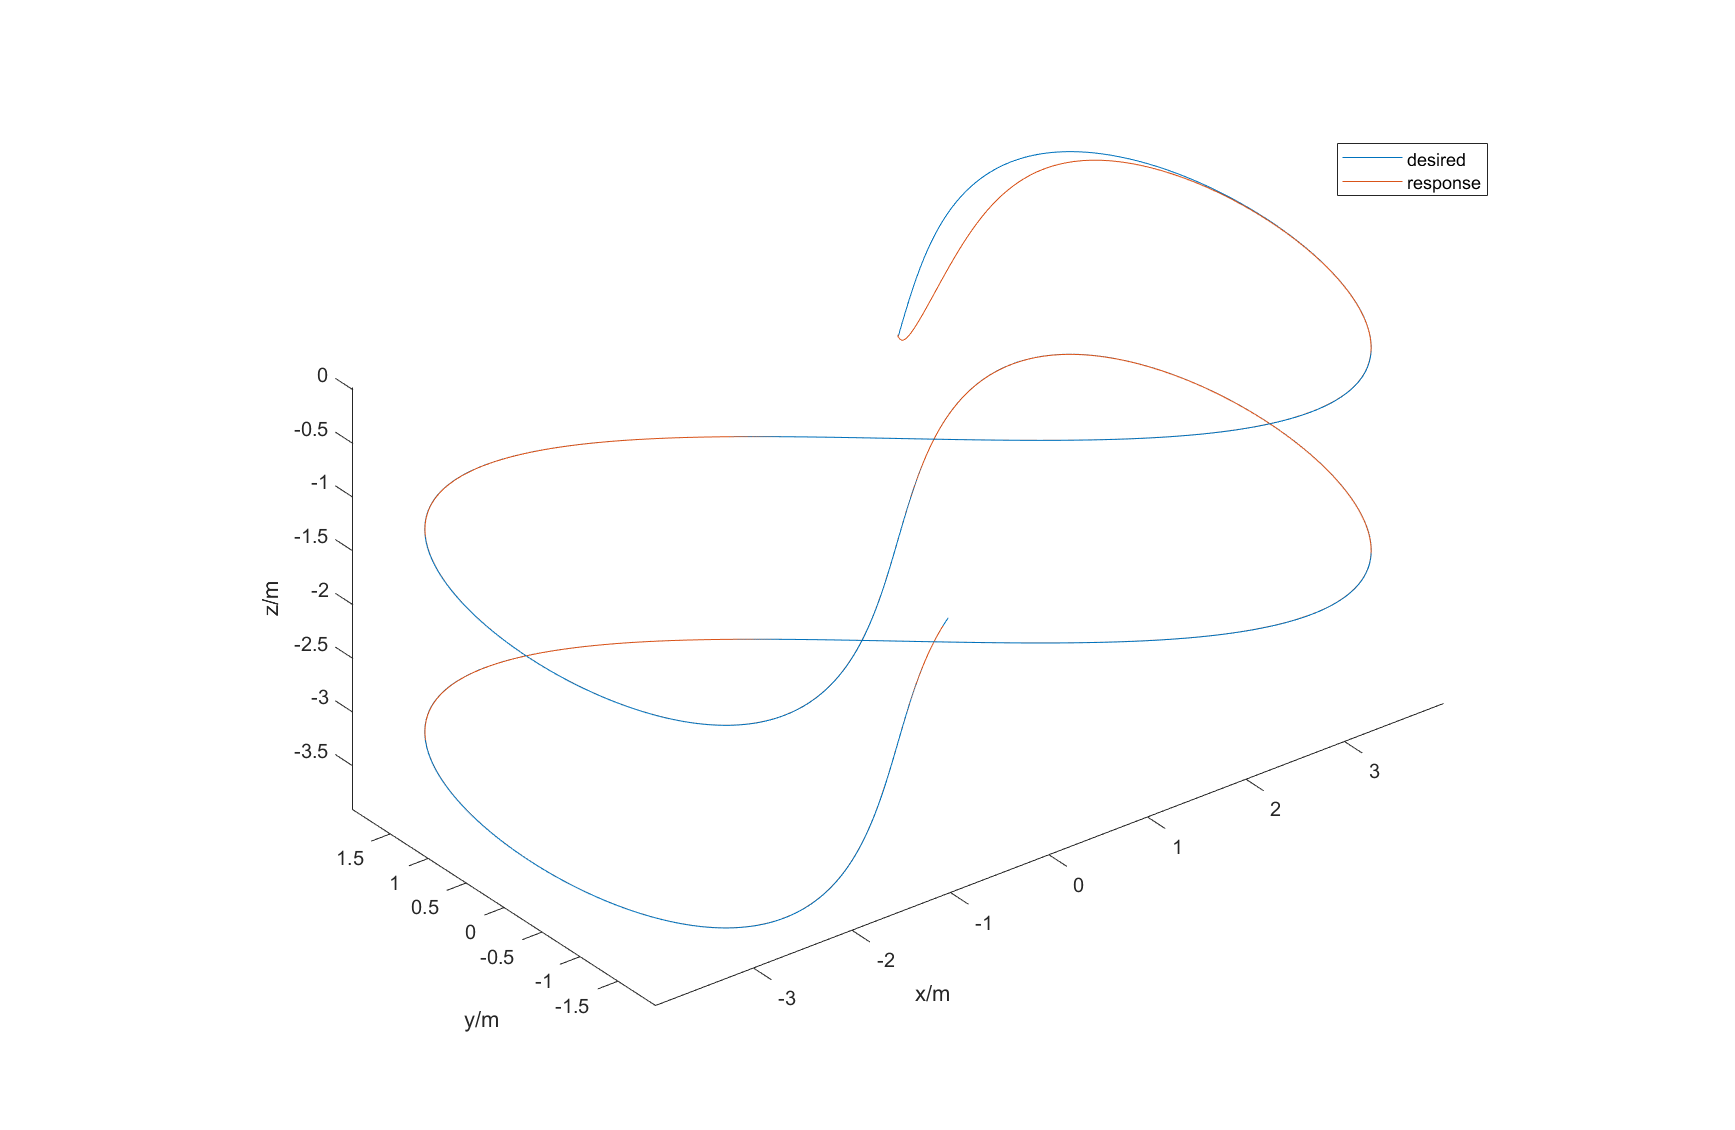
\includegraphics[width=0.7\textwidth]{result2.png}
    \caption{三维的跟踪效果}
    \label{fig:result2}
  \end{figure}

  \begin{figure}[!h]
    \centering
    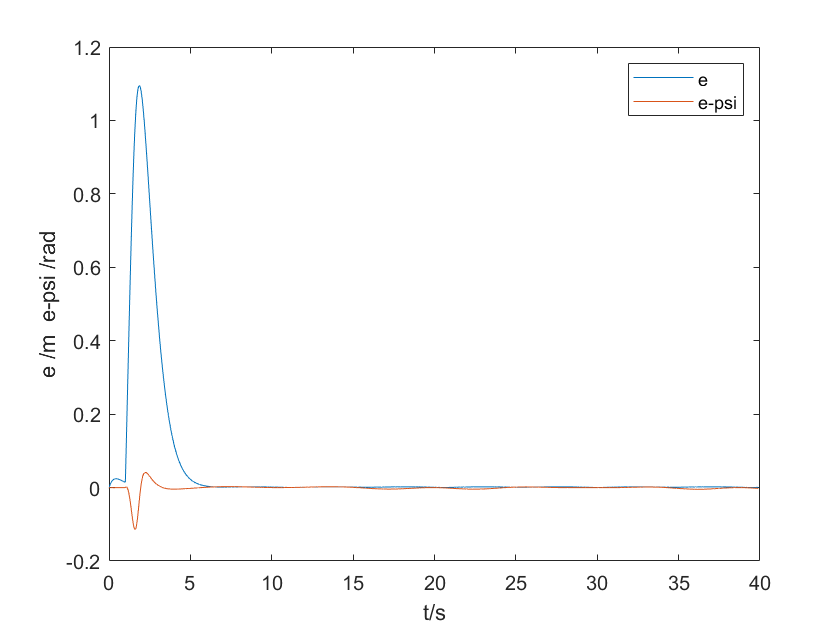
\includegraphics[width=0.7\textwidth]{result3.png}
    \caption{量化跟踪效果}
    \label{fig:result3}
  \end{figure}